\subsection{Analysis: Symbolic Execution}

As we have discussed in the previous subsection, there are two types of approaches when we speak about verification:
\begin{itemize}
    \item \definition{Static Analysis}. It analyzes the source code, and each analyzer targets a fixed set of hard-coded (pre-defined, not custom) properties. It is entirely automatic, and the output reports two types of results: safe (no issues) and unsafe (potential problems). Also, the \textbf{analysis is made on generic (or symbolic) inputs}.
    
    The properties that we have mentioned are safety properties, such as:
    \begin{itemize}
        \item No \emph{overflow} for integer variables
        \item No \emph{type errors}
        \item No \emph{null-pointer} dereferencing
        \item No \emph{out-of-bound} array accesses
        \item No \emph{race conditions}
        \item No \emph{useless assignments}
        \item No \emph{usage of undefined variables}
        \item No \emph{execution of specific paths}
    \end{itemize}
    
    \item Testing (dynamic analysis) is made at runtime and is related to the software's behavior during execution. The analysis is also made on specific inputs.
\end{itemize}
Using the static analysis, we can use the symbolic execution.

\begin{definitionbox}\label{def: symbolic execution}
    \definition{Symbolic Execution} (also symbolic evaluation) \textbf{analyses a program to determine what inputs cause each part of a program to execute}.
\end{definitionbox}

\noindent
The \textbf{symbolic execution} analyzes actual source code and \textbf{reachability} and \textbf{path feasibility} properties. It is automatic and may fail to explore all possible paths. Sometimes, it is used to support testing.

The checked properties by the static analysis can be of different types:
\begin{itemize}
    \item \definition{Reachability}. Does some program execution reach location $L$ (generic line of code) in S (source code)? With the reachability property, the symbolic execution tries:
    \begin{itemize}
        \item To \textbf{verify} that $L$ \textbf{cannot be reached};
        \item Or \textbf{spots the condition under which} $L$ \textbf{can be reached}.
    \end{itemize}
    For example, in the following code:
    \begin{lstlisting}
...
k:      try {
k+1:        ...
L-1:    } catch (e) {
L:          /* error */
...     }\end{lstlisting}
    Static analysis checks the reachability properties and verifies that $L$ cannot be reached, or discovers the condition under which $L$ can be reached.
    
    \item \definition{Path Feasibility}. Is the given path $p$ feasible? With the path feasibility property, the symbolic execution tries:
    \begin{itemize}
        \item To \textbf{verify} that $p$ \textbf{cannot be executed};
        \item Or \textbf{spots the condition under which} $p$ \textbf{can be executed}.
    \end{itemize}
    Then $p$ will be:
    \begin{equation*}
        p = < 0, 1, \dots, k, \dots, n >
    \end{equation*}
\end{itemize}
Symbolic execution \textbf{executes programs on symbolic values}. Each symbolic value has its \textbf{symbolic states}, which keep track of the variables' (symbolic) values. The inputs are initialized with symbolic (generic) values.

\highspace
In the following example we can see a complete example of symbolic execution. But before we do, let us introduce some \underline{\textbf{limitations}} of this methodology.
\begin{itemize}
    \item The \textbf{path conditions may be too complex for constraint solvers}. Because solvers are very good at checking linear constraints, but it is harder for them to reason about non-linear arithmetic, bit-wise operations, string manipulation, etc.
    
    \item It is \textbf{impossible} or \textbf{difficult to use when the number of paths to be explored is infinite} or \textbf{huge}. For example, unbounded loops give rise to infinite sets of paths. Although the set of paths is finite, checking all loops is expensive and impractical.
    
    \item Finally, there may be \textbf{external code}. Then the sources are not available, such as a precompiled library, or the behavior is unknown to the solver.
\end{itemize}
\begin{examplebox}\label{example: Symbolic Execution}
    \begin{enumerate}
        \item First we introduce the annotation:
        \begin{lstlisting}
void foo(int x, int y) {
    ...\end{lstlisting}
        \begin{center}
            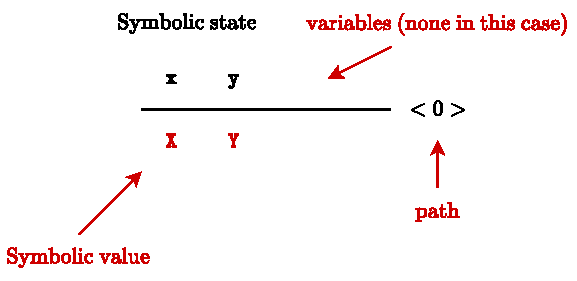
\includegraphics[width=.7\textwidth]{img/symbolic-state-1.pdf}
        \end{center}


        \item We introduce a local variable:
        \begin{lstlisting}
void foo(int x, int y) {
    int z := x\end{lstlisting}
        \begin{center}
            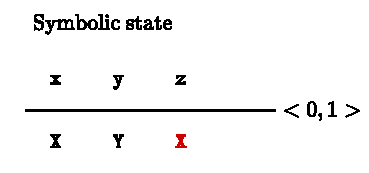
\includegraphics[width=.5\textwidth]{img/symbolic-state-2.pdf}
        \end{center}


        \item We introduce a condition. A \textbf{path condition} $\pi$ represents a constraint on a path:
        \begin{lstlisting}
void foo(int x, int y) {
    int z := x
    if (z < y)\end{lstlisting}
        \begin{itemize}
            \item if condition true
            \begin{center}
                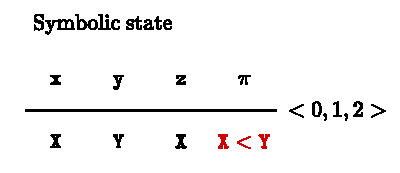
\includegraphics[width=.5\textwidth]{img/symbolic-state-3.pdf}
            \end{center}

            \item if condition false
            \begin{center}
                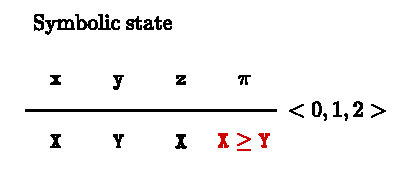
\includegraphics[width=.5\textwidth]{img/symbolic-state-4.pdf}
            \end{center}
        \end{itemize}


        \item \textbf{Execution continues along feasible paths}. In this case, the path condition $\pi$ is satisfiable:
        \begin{lstlisting}
void foo(int x, int y) {
    int z := x
    if (z < y)
        z := z*2\end{lstlisting}
        \begin{center}
            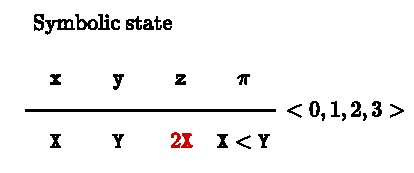
\includegraphics[width=.5\textwidth]{img/symbolic-state-5.pdf}
        \end{center}


        \item Another if condition:
        \begin{lstlisting}
void foo(int x, int y) {
    int z := x
    if (z < y)
        z := z*2
    if (x < y && z >= y)\end{lstlisting}
        \begin{itemize}
            \item if condition true
            \begin{center}
                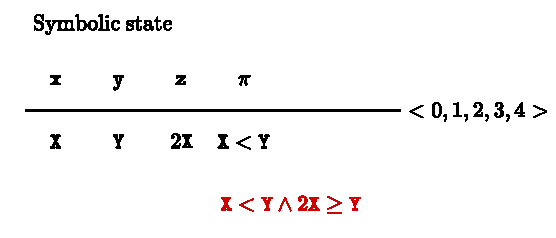
\includegraphics[width=.6\textwidth]{img/symbolic-state-6.pdf}
            \end{center}

            \item if condition false
            \begin{center}
                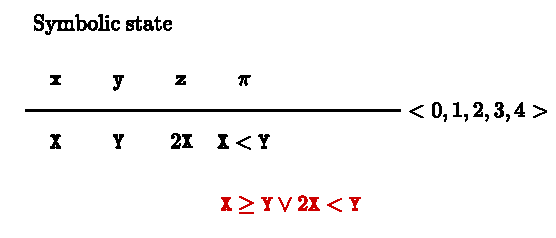
\includegraphics[width=.6\textwidth]{img/symbolic-state-7.pdf}
            \end{center}
        \end{itemize}


        \item Possible outcomes of symbolic execution:
        \begin{lstlisting}
void foo(int x, int y) {
    int z := x
    if (z < y)
        z := z*2
    if (x < y && z >= y)
        print(z)
}\end{lstlisting}
        \begin{enumerate}
            \item \textcolor{Green3}{\textbf{Satisfiable}} exit ($\pi$ is satisfiable): every satisfying assignment to variables in $\pi$ is an \textbf{input that satisfies the given property in a concrete execution}.
            \begin{center}
                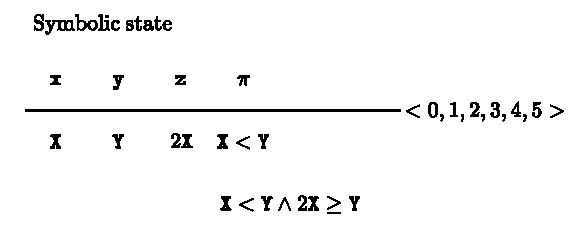
\includegraphics[width=.6\textwidth]{img/symbolic-state-8.pdf}
            \end{center}


            \item \textcolor{Red2}{\textbf{Unsatisfiable}} exit ($\pi$ is not satisfiable): the given \textbf{property cannot be satisfied by any concrete execution}.
            \begin{center}
                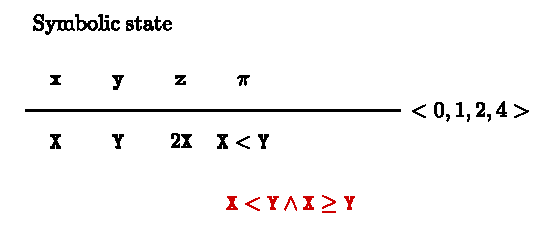
\includegraphics[width=.6\textwidth]{img/symbolic-state-9.pdf}
            \end{center}
        \end{enumerate}
    \end{enumerate}
    Finally, we can draw the \definition{Execution Tree}. The execution paths can be collected in an execution tree, where end states are marked as \texttt{SAT} or \texttt{UNSAT}.
    \begin{center}
        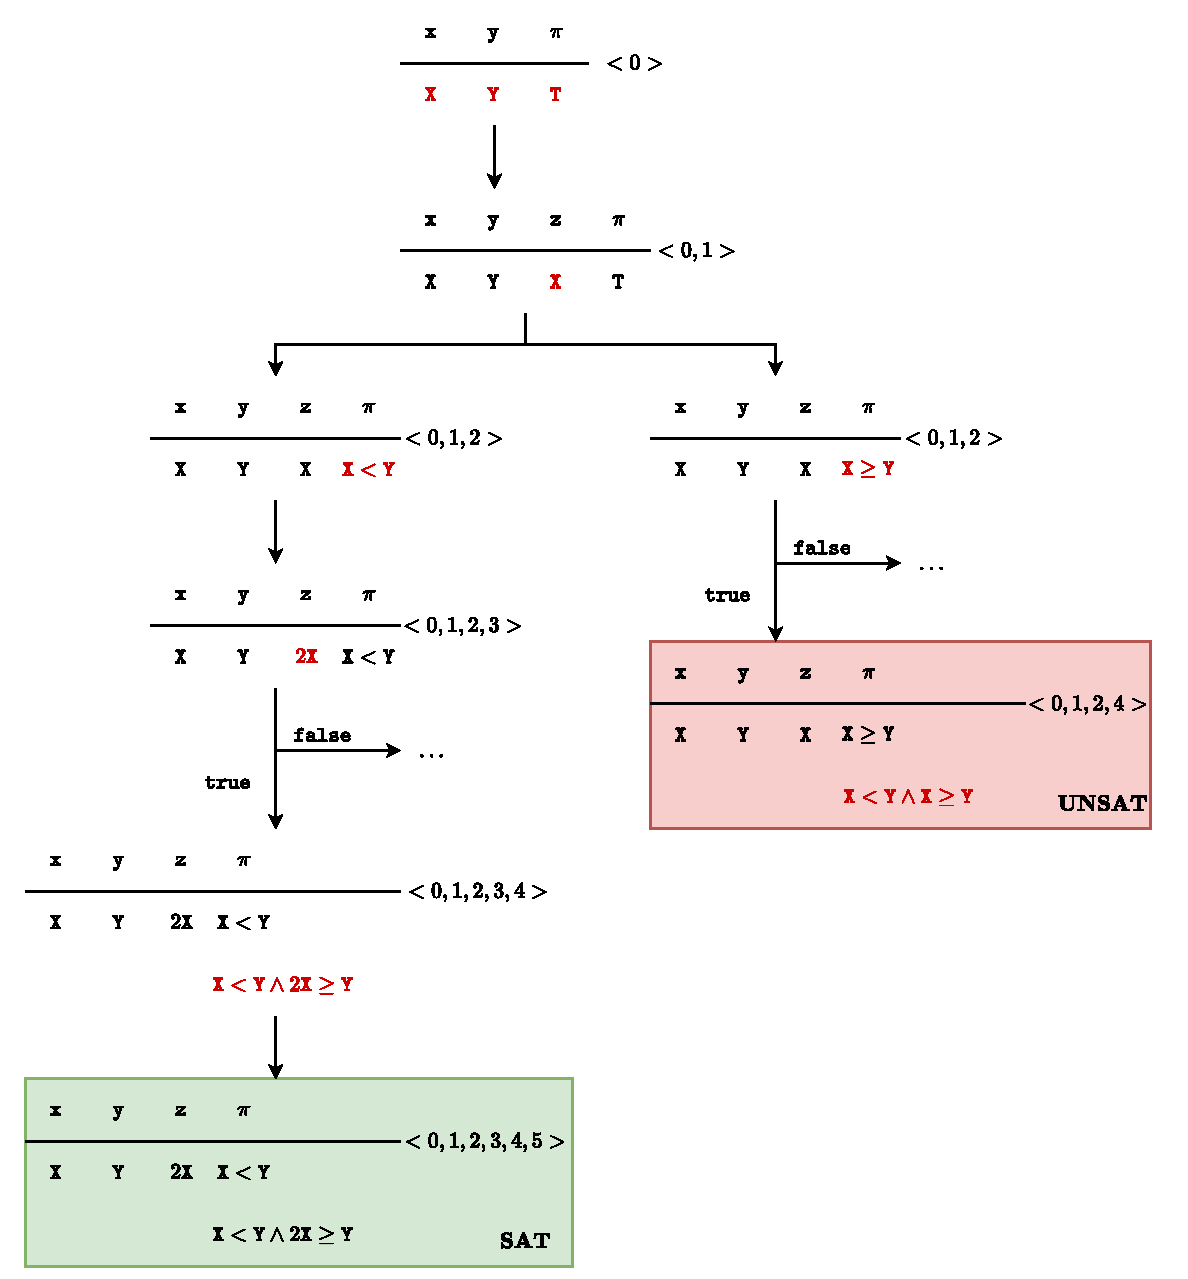
\includegraphics[width=\textwidth]{img/symbolic-state-10.pdf}
    \end{center}
    To view the tree in high resolution, scan (or click) the QR code below.
    \begin{center}
        \qrcode{https://github.com/PoliMI-HPC-E-notes-projects-AndreVale69/HPC-E-PoliMI-university-notes/tree/main/software-engineering-for-hpc/notes/img/symbolic-state-10.pdf}
    \end{center}
\end{examplebox}